\documentclass{article}
\usepackage{graphicx, amsmath}
\graphicspath{ {./images/} }

\title{HW 10.2.-10.3. Solutions}
\author{Principles of Microeconomics}
\date{\today}

\begin{document}

\maketitle

\subsection*{QuickQuiz}

\begin{enumerate}
\setcounter{enumi}{2}

\item (a) --

	\begin{center}
	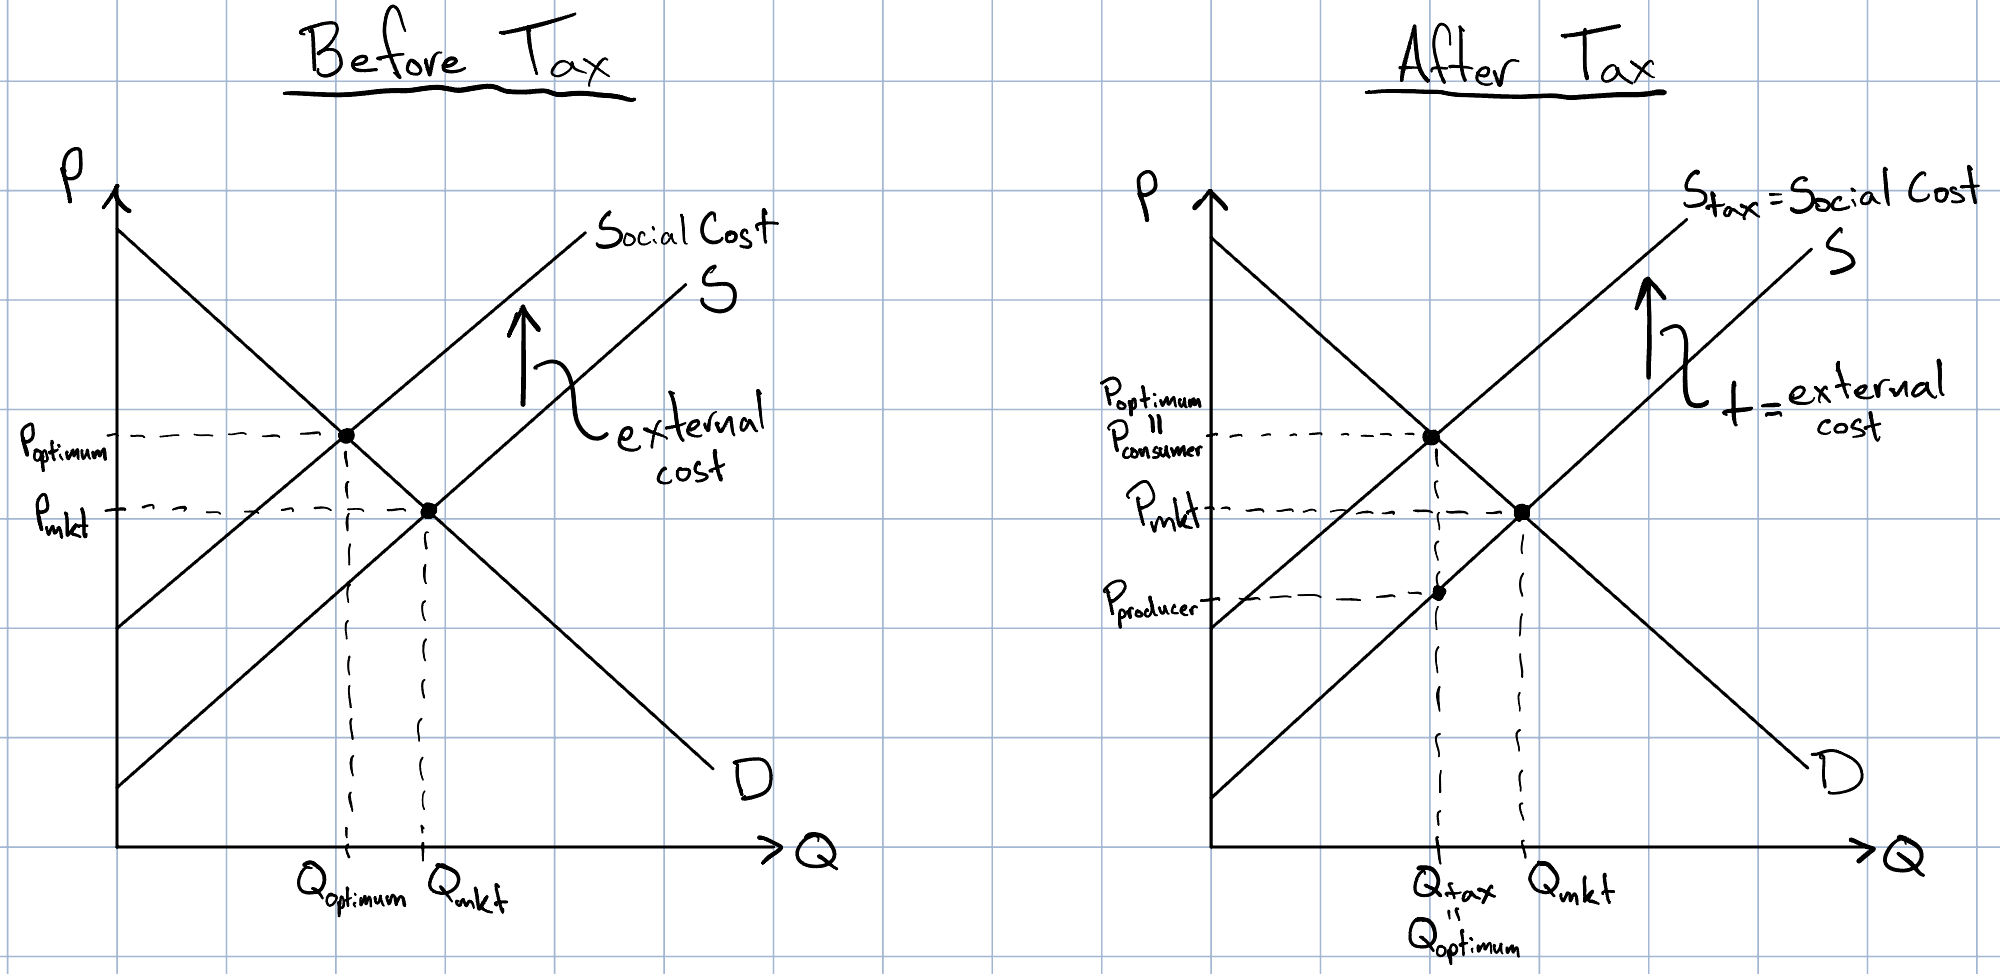
\includegraphics[width = \textwidth]{qq3}
	\end{center}

\item (d) -- Corrective taxes make markets more efficient. That means they increase total surplus, not deadweight loss.

\item (b) --

	\begin{align*}
	Tax \ Revenue &= Q_{tax} \cdot t \\
	\$25,000 &= 500t \\
	50 &= t
	\end{align*}
	
\item (c) -- Every other answer is a reason to prefer a corrective tax. 

\end{enumerate}

\subsection*{Problems and Applications}

\begin{enumerate}
\setcounter{enumi}{3}

\item 

	\begin{enumerate}

	\item It's possible that some firms can reduce pollution at lower costs than others. If that's the case, the lowest cost way for society to reduce pollution would be for those firms to reduce their pollution more, and the other firms to reduce their pollution less. 
	
	\item If the command-and-control approach mandates a uniform reduction, then the firms with lower reduction costs aren't reducing their pollution more and the firms with higher reduction costs aren't reducing their pollution less. 
	
	\item Corrective taxes and tradable pollution permits force firms to pay for each unit of pollution they create. Firms that can reduce pollution at a lower cost will reduce their pollution substantially to avoid paying the tax or buying permits. Firms that can only reduce pollution at a high cost will reduce their pollution less and pay more tax or buy more permits.

	\end{enumerate}
	
\item

	\begin{enumerate}
	
	\item Each Whovillian will consume four bottles because their willingness to pay is only greater than \$1.50 for the first bottles. Their consumer surplus is
		\[ CS = 5 - 1.5 + 4 - 1.5 + 3 - 1.5 + 2 - 1.5 = 8. \]
		
	\item The social cost of each bottle is now \$2.50. That means total surplus per person is 
		\[TS = 5 - 2.5 + 4 - 2.5 + 3 - 2.5 + 2 - 2.5 = 4. \]
		
	\item The welfare that Cindy generates increases to 
		\[ TS = 5 - 2.5 + 4 - 2.5 + 3 - 2.5 = 4.5. \]
		As a result, total surplus in Whoville increases.
		
	\item Now the private cost of each bottle is \$2.50. That means each Whovillian will only consume three bottles. 
		\begin{align*}
		CS &= 5 - 2.5 + 4 - 2.5 + 3 - 2.5 = 4.5 \\
		External \ Cost &= 3(1) = 3 \\
		Government \ Revenue &= 3(1) = 3 \\
		TS &= CS - External \ Cost + Gov't \ Revenue \\
		&= 4.5 - 3 + 3 = 4.5
		\end{align*}
		
	\item I would support the mayor's policy. It increases total surplus per person.
	
	\end{enumerate}

\end{enumerate}

\end{document}